  \let\negmedspace\undefined
\let\negthickspace\undefined
\documentclass[journal]{IEEEtran}
\usepackage[a5paper, margin=10mm, onecolumn]{geometry}
\usepackage{lmodern} 
\usepackage{tfrupee} 

\setlength{\headheight}{1cm} 
\setlength{\headsep}{0mm}    

\usepackage{gvv-book}
\usepackage{gvv}
\usepackage{cite}
\usepackage{amsmath,amssymb,amsfonts,amsthm}
\usepackage{algorithmic}
\usepackage{graphicx}
\usepackage{textcomp}
\usepackage{xcolor}
\usepackage{txfonts}
\usepackage{listings}
\usepackage{enumitem}
\usepackage{mathtools}
\usepackage{gensymb}
\usepackage{comment}
\usepackage[breaklinks=true]{hyperref}
\usepackage{tkz-euclide} 
\usepackage{listings}                                      
\def\inputGnumericTable{}                                 
\usepackage[latin1]{inputenc}                                
\usepackage{color}                                            
\usepackage{array}                                            
\usepackage{longtable}
\usepackage{multicol}
\usepackage{calc}                                             
\usepackage{multirow}                                         
\usepackage{hhline}                                           
\usepackage{ifthen}                                           
\usepackage{lscape}
\begin{document}

\bibliographystyle{IEEEtran}
\vspace{3cm}

\title{1.9.20}
\author {EE25BTECH11031 - Sai Sreevallabh}
% \maketitle
% \newpage
% \bigskip
{\let\newpage\relax\maketitle}

\renewcommand{\thefigure}{\theenumi}
\renewcommand{\thetable}{\theenumi}
\setlength{\intextsep}{10pt} % Space between text and floats


\numberwithin{equation}{enumi}
\numberwithin{figure}{enumi}
\renewcommand{\thetable}{\theenumi}

\textbf{Question: }\\

Find the point on the Y-Axis which is equidistant from the points $\brak{5,-2}$ and $\brak{-3,2}$\\ 

\textbf{Solution: }\\

Given points are\\
\begin{align}
    \vec{A}=\myvec{5\\-2} \ \text{and}\  \vec{B}=\myvec{-3\\2}
\end{align}

Let $\vec{P}$ be a point on the Y-Axis. \\
\begin{align}
    \vec{P}=\myvec{0\\y}
\end{align}

$\vec{P}$ is equidistant from both $\vec{A}$ and $\vec{B}$. Hence the norms of vectors $\vec{P}-\vec{B}$ and $\vec{P}-\vec{A}$ are equal. 

\begin{align}
    \norm{\vec{P}-\vec{B}} =& \norm{\vec{P}-\vec{A}}\\
    \implies  \norm{\vec{P}-\vec{B}}^2 =& \norm{\vec{P}-\vec{A}}^2\\
    \implies \norm{\vec{P}}^2 - 2\vec{P}^\top\vec{A} + \vec{A}^2 =& \norm{\vec{P}}^2 - 2\vec{P}^\top\vec{B} + \vec{B}^2
\end{align}

Simplification of the above results in:
\begin{align}
    \brak{\vec{A}-\vec{B}}^\top\vec{P} = \frac{\norm{A}^2 - \norm{B}^2}{2} 
\end{align}

\begin{align}
    \because \vec{P} = y\vec{e_2}   
\end{align}

where, $\vec{e_2} = \myvec{0\\1}$.

\begin{align}
    y = \frac{\norm{A}^2-\norm{B}^2}{2\brak{\vec{A}-\vec{B}}^\top\vec{e_2}}
\end{align}

Substituting the values of $\vec{A}$ and $\vec{B}$:

\begin{align}
    y = \frac{\norm{\myvec{5\\-2}}^2 - \norm{\myvec{-3 \\2}}^2}{2\myvec{8 & -4}\myvec{0\\1}}
\end{align}

\begin{align}
    y = -2
\end{align}

$\therefore$ The point on the y-axis that is equidistant from the given two points is $\vec{P}$ = $\myvec{0\\-2}$.

\begin{figure}[H]
    \centering
    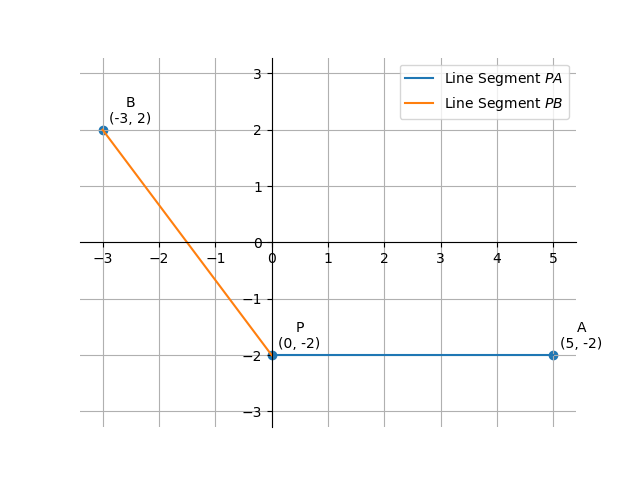
\includegraphics[width=1\columnwidth]{Figs/plot(py).png}
\end{figure}

\end{document}
